\documentclass{ieeeaccess}
\usepackage{cite}
\usepackage{amsmath,amssymb,amsfonts}
\usepackage{algorithm,algorithmic}
\usepackage{graphicx}
\usepackage{textcomp}
\usepackage{bm}
\usepackage{float}
\makeatletter
\AtBeginDocument{\DeclareMathVersion{bold}
    \SetSymbolFont{operators}{bold}{T1}{times}{b}{n}
    \SetSymbolFont{NewLetters}{bold}{T1}{times}{b}{it}
    \SetMathAlphabet{\mathrm}{bold}{T1}{times}{b}{n}
    \SetMathAlphabet{\mathit}{bold}{T1}{times}{b}{it}
    \SetMathAlphabet{\mathbf}{bold}{T1}{times}{b}{n}
    \SetMathAlphabet{\mathtt}{bold}{OT1}{pcr}{b}{n}
    \SetSymbolFont{symbols}{bold}{OMS}{cmsy}{b}{n}
    \renewcommand\boldmath{\@nomath\boldmath\mathversion{bold}}}
\makeatother

\def\BibTeX{{\rm B\kern-.05em{\sc i\kern-.025em b}\kern-.08em
T\kern-.1667em\lower.7ex\hbox{E}\kern-.125emX}}

%Your document starts from here ___________________________________________________
\begin{document}
\history{Date of publication xxxx 00, 0000, date of current version xxxx 00,
    0000.}
\doi{10.1109/ACCESS.2024.0429000}

\title{Vega: Intelligent Chatbot Platform for Internet of Things and Embedded Systems Development}
% //TODO: ask about IEEE membership
\author{\uppercase{Harith Al-Safi}, \IEEEmembership{Fellow, IEEE},
    \uppercase{Harith Ibrahim}, and Paul Steenson,
    \IEEEmembership{SeniroMember, IEEE}}

\address{School of Electronics and Electrical Engineering, University of Leeds,
    Leeds LS2 9JT, U.K}
\tfootnote{This paragraph of the first footnote will contain support
    information, including sponsor and financial support acknowledgment. For
    example, ``This work was supported in part by the U.S. Department of
    Commerce under Grant BS123456.''}

\markboth
{Author \headeretal: Preparation of Papers for IEEE TRANSACTIONS and JOURNALS}
{Author \headeretal: Preparation of Papers for IEEE TRANSACTIONS and JOURNALS}

\corresp{Corresponding author: Harith Al-Safi (e-mail:
    harith.alsafi@gmail.com).}

% TODO: make verbs past tense
% alternative word to 'non-technical' users
% use Vega in abstract 
\begin{abstract}
    Large language models (LLMs) have revolutionized natural language
    processing, yet their potential in Internet of Things (IoT) and embedded systems (ESys) applications remains largely untapped. Traditional IoT interfaces often require specialized
    knowledge, creating barriers for non-technical users. We present a modular
    system that leverages LLMs to enable intuitive, natural language control of IoT
    devices, specifically a Raspberry Pi (RPi) connected to various sensors and
    devices. Our solution comprises three key components: a physical circuit with
    input and output devices, an RPi integrating a control server, and a web
    application integrating LLM logic. Users interact with the system through
    natural language commands, which the LLM interprets to call appropriate
    commands for the RPi. The RPi executes these instructions on the connected
    circuit, with outcomes communicated back to the user via LLM-generated
    responses. We empirically evaluate our system's performance across a range of
    task complexities and user scenarios, demonstrating its ability to handle
    complex, conditional logic without additional RPi-level coding. Our findings
    reveal that LLM-driven IoT control can effectively bridge the gap between
    complex device functionality and user-friendly interaction. We discuss the
    system's scalability, exploring its potential applications in diverse settings
    such as smart homes, industrial monitoring, and educational environments. By
    enabling natural language interaction with IoT devices, our approach not only
    enhances accessibility for non-technical users but also opens new avenues for
    creative and intelligent IoT applications. This research contributes to the
    growing body of work on interactive intelligent systems for IoT, offering
    insights into the design and implementation of LLM-integrated IoT interfaces.
\end{abstract}

\begin{keywords}
    Enter key words or phrases in alphabetical
    order, separated by commas. Autocorrelation, beamforming, communications
    technology, dictionary learning, feedback, fMRI, mmWave, multipath, system
    design, multipath, slight fault, underlubrication fault.
\end{keywords}

\titlepgskip=-21pt

\maketitle

\section{Introduction}
\label{sec:introduction}

Large language models (LLMs) have revolutionized natural language processing, demonstrating unprecedented capabilities in understanding and generating human-like text \cite{10.1145/3641289}. However, their potential in Internet of Things (IoT) and embedded systems (ESys) applications remains largely untapped. IoT systems have become increasingly prevalent across various domains, from smart homes to industrial automation \cite{8355897}. Despite their widespread adoption, developing and interacting with IoT systems often requires specialized knowledge and programming skills, creating significant barriers for non-technical users \cite{10.1145/3447526.3472036}.

Traditional IoT interfaces typically rely on graphical user interfaces (GUIs) or specific programming languages, which can be challenging for users without technical expertise \cite{10.1145/3447526.3472036}. This limitation hinders the widespread adoption and utilization of IoT technologies, particularly in scenarios where rapid deployment and intuitive interaction are crucial. While research has been conducted on natural language interfaces for IoT, the application of advanced language models to IoT control and interaction remains an underexplored area \cite{KASSAB2020102663}.

To address these challenges, we propose Vega, an intelligent chatbot platform that leverages LLMs to enable intuitive, natural language control of IoT devices. Our system focuses on a Raspberry Pi (RPi) connected to various sensors and devices as a representative IoT setup. By integrating LLMs with IoT infrastructure, we aim to bridge the gap between complex device functionality and user-friendly interaction, allowing users to control and query IoT systems using everyday language.

Our research builds upon recent advancements in LLMs, specifically OpenAI's GPT-based models \cite{OpenAI_GPT}, which utilize transformer neural network architectures to capture context and relationships within text data. By applying these powerful language understanding capabilities to IoT interaction, we aim to create a more accessible and flexible approach to device control and monitoring. Our approach not only enhances accessibility for non-technical users but also opens new avenues for creative and intelligent IoT applications, addressing the standardization challenges highlighted in the literature \cite{7821686}.

Vega's architecture comprises three key components: a physical circuit with input and output devices, an RPi integrating a control server, and a web application incorporating LLM logic. This modular design allows for flexibility and scalability, enabling the system to adapt to various IoT scenarios and user requirements \cite{taylor2010software}. By utilizing the RPi as a central hub, we can leverage its versatility and widespread adoption in the IoT community \cite{8067944}.

The main contributions of this paper are as follows:

\begin{enumerate}
    \item We present a modular architecture that integrates LLMs with IoT systems, specifically designed for natural language interaction with RPi-based setups.
    \item We develop a novel approach for translating natural language commands into executable instructions for IoT devices, capable of handling complex, conditional logic without additional RPi-level coding.
    \item We implement and evaluate a prototype system demonstrating the feasibility and effectiveness of LLM-driven IoT control across a range of task complexities and user scenarios.
    \item We provide insights into the scalability and potential applications of our approach in diverse settings such as smart homes, industrial monitoring, and educational environments.
\end{enumerate}

The rest of this paper is organized as follows: Section II provides background information and discusses related work in IoT interfaces and natural language processing. Section III details our methodology, including the overall system architecture, physical circuit design, RPi configuration, and web application implementation. Section IV presents our experimental setup, results, and analysis, showcasing the system's performance in handling complex commands and its potential real-world applications. Finally, Section V concludes the paper and outlines directions for future research.

\section{Background and Related Work}
\label{sec:background}

\subsection{NLP in IoT and ESys}
\subsection{LLM's in industrial applications}
\subsection{Accessible Chatbot }



\section{Methodology}
\label{sec:methodology}

Hi \cite{taylor2010software} how are you

\subsection{Overall Architecture}
\Figure[t!](topskip=0pt, botskip=0pt, midskip=0pt)[width=\textwidth]{{figures/fig1-ab.png}}
{ \textbf{Magnetization as a function of applied field.
It is good practice to explain the significance of the figure in the caption.}\label{fig1}}

% \begin{table}
%     \caption{\textbf{Units for Magnetic Properties}}
%     \label{table}
%     \setlength{\tabcolsep}{2pt}
%     \begin{tabular}{|p{65pt}|p{35pt}|p{45pt}|p{75pt}|}
%     \hline
%     Module Name&
%     Language&
%     Framework&
%     Main Libraries \\
%     \hline
%     Webapp interface&
%     Typescript&
%     React.js&
%     RadixUI,TailwindCSS\\
%     Webapp logic&
%     Typescript&
%     Next.js, Node.js&
%     OpenAI\\
%     \hline

%     \end{tabular}
%     \label{tab1}
%     \end{table}

\subsection{Physical Circuit Design}

\Figure[t!](topskip=0pt, botskip=0pt,
midskip=0pt)[width=\textwidth]{{figures/fig5.png}}
{ \textbf{Soldered physical circuit connected to the RPi}\label{fig2}}

\subsection{Raspberry Pi Design}
\begin{table}
    \caption{\textbf{Physical devices defined on the Control Server, which are then supplied to the LLM}}
    \label{table1}
    \setlength{\tabcolsep}{3pt}
    \begin{tabular}{|p{30pt}|p{25pt}|p{180pt}|}
        \hline
        \textbf{Symbol} &
        \textbf{Type}   &
        \textbf{Description}                                             \\
        \hline
        ULTS   &
        Input  &
        Ultrasonic Distance Sensor in 'cm'                      \\
        \hline
        CAM    &
        Input  &
        Camera device for picture input                         \\
        \hline
        GPS    &
        Input  &
        GPS device for longitude and latitude coordinates       \\
        \hline
        TMP    &
        Input  &
        Temperature sensor giving response in degree celcuis    \\
        \hline
        FAN    &
        Output &
        12V fan controled by a digital GPIO pin through a relay \\
        \hline
        LCD    &
        Output &
        I2C LCD for displaying strings                          \\
        \hline
        SRV    &
        Output &
        Servo motor rotates using PWM to a given angles         \\
        \hline
        LED1   &
        Output &
        Yellow LED light                                        \\
        \hline
        LED2   &
        Output &
        Red LED light                                           \\
        \hline
        LED3   &
        Output &
        Blue LED light                                          \\
        \hline
    \end{tabular}
\end{table}

\begin{table}
    \caption{\textbf{Defined functions on the Control Server, called by the LLM based on user input, executes on the RPi and processed on the webapp}}
    \label{table2}
    \setlength{\tabcolsep}{3pt}
    \begin{tabular}{|p{80pt}|p{70pt}|p{85pt}|}
        \hline
        \textbf{Function}    &
        \textbf{Description} &
        \textbf{Use Case} \\
        \hline
        set\underbar{ }led   &
        Toggles specefic LED &
        "Turn on yellow LED" \\
        \hline 
        set\underbar{ }fan   &
        Toggles fan on or off&
        "Turn on the fan" \\
        \hline
        get\underbar{ }recorded\underbar{ }sensor\underbar{ }data   &
        Gets interval sensor data from database&
        "Plot me the distance data in last 30 seconds" \\
        \hline
        get\underbar{ }raspberry\underbar{ }stats   &
        Gets CPU, RAM, Disk of RPi&
        "What is the currrent disk usage" \\
        \hline
        capture\underbar{ }image&
        Capture and upload image to Imgur&
        "Capture an image, does it contain a pen?" \\
        \hline
        get\underbar{ }connected\underbar{ }devices    &
        Fetches the data of connected devices&
        "What is the current humidity and temperature" \\
        \hline
        get\underbar{ }location\underbar{ }   &
        Gets the current  \newline
        location from GPS&
        "From the location are we currently in Leeds?" \\
        \hline
        set\underbar{ }servo\underbar{ }angles    &
        Turn servo to certain angle &
        "Turn the servo to 10 then 180 degrees" \\
        \hline
    \end{tabular}
\end{table}
\Figure[t!](topskip=0pt, botskip=0pt,
midskip=0pt)[scale=0.4]{{figures/fig6.png}}
{ \textbf{Architecture design of the RPi control server}\label{fig3}}

\subsection{Web App User Interface}
\Figure[t!](topskip=0pt, botskip=0pt,
midskip=0pt)[width=\textwidth]{{figures/fig9.png}}
{ \textbf{Webapp user interface implementation}\label{fig4}}

\subsection{Web App LLM Logic}
\Figure[t!](topskip=0pt, botskip=0pt,
midskip=0pt)[width=0.99\columnwidth]{{figures/fig12.png}}
{ \textbf{Evaluation metrics for the functions defined earlier in .}\label{fig7}}

\Figure[t!](topskip=0pt, botskip=0pt,
midskip=0pt)[width=\textwidth]{{figures/fig13.png}}
{ \textbf{Webapp logic design}\label{fig5}}

\section{Experiment and Results}
\label{sec:experiment}

\subsection{Complex Commands In Action}
\Figure[t!](topskip=0pt, botskip=0pt,
midskip=0pt)[width=\textwidth]{{figures/fig30.png}}
{ \textbf{System case studies}\label{fig6}}


\subsection{Automated Evaluation}
\Figure[t!](topskip=0pt, botskip=0pt, midskip=0pt)[scale=0.48]{{figures/fig15.png}}
{ \textbf{Magnetization as a function of applied field.
It is good practice to explain the significance of the figure in the caption.}\label{fig6}}
\subsection{Result Analysis}

% define how complexity is measured 
\Figure[t!](topskip=0pt, botskip=0pt,
midskip=0pt)[width=0.99\columnwidth]{{figures/fig17.png}}
{ \textbf{Evaluation metrics for the functions defined earlier in .}\label{fig7}}

\Figure[t!](topskip=0pt, botskip=0pt,
midskip=0pt)[width=0.99\columnwidth]{{figures/fig18.png}}
{ \textbf{Message complexity against the number of functions called per message.}\label{fig8}}

% change this to percentage
\Figure[t!](topskip=0pt, botskip=0pt,
midskip=0pt)[width=0.99\columnwidth]{{figures/fig19.png}}
{ \textbf{Message complexity against all evaluation metrics and most importantly the success rate.}\label{fig9}}


% \Figure[t!](topskip=0pt, botskip=0pt,
% midskip=0pt)[width=0.99\columnwidth]{{figures/fig26.png}}
% { \textbf{Magnetization as a function of applied field.
%         It is good practice to explain the significance of the figure in the
%         caption.}\label{fig9}}

% change the temperature its wrong
\Figure[t!](topskip=0pt, botskip=0pt,
midskip=0pt)[width=0.99\columnwidth]{{figures/fig36.png}}
{ \textbf{Success rate against message complexity and temperature of the LLM.}\label{fig10}}

\Figure[t!](topskip=0pt, botskip=0pt,
midskip=0pt)[width=0.99\columnwidth]{{figures/fig37.png}}
{ \textbf{Success rate against message complexity and Top P of the LLM.}\label{fig11}}

\Figure[t!](topskip=0pt, botskip=0pt,
midskip=0pt)[width=0.80\columnwidth]{{figures/fig34.png}}
{ \textbf{What types of errors occured throughout testing.}\label{fig12}}

\Figure[t!](topskip=0pt, botskip=0pt,
midskip=0pt)[width=0.99\columnwidth]{{figures/fig35.png}}
{ \textbf{Success rate of different tones of the same message.}\label{fig13}}

\subsection{Real Life Applicability}

\section{Conclusion and future work}
\label{sec:conclusion}

\section*{Acknowledgment}

\bibliographystyle{unsrt}
\bibliography{refs}

\begin{IEEEbiography}[{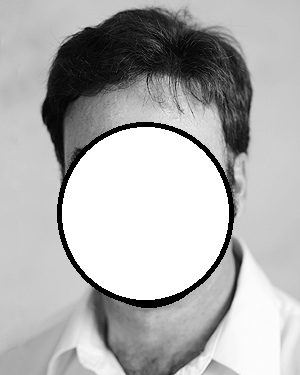
\includegraphics[width=1in,height=1.25in,clip,keepaspectratio]{author1.png}}]{Harith Al-Safi} received the BEng industrial degree in Electronics and Computer Engineering from
    the University of Leeds, Leeds, in 2024. From 2022 to 2023, he was an IoT Software Engineer at Johnson Controls. He is currently pursuing a Graduate Software Developer role at BT Group. His research interests include IoT, embedded systems, and machine learning.
\end{IEEEbiography}

\begin{IEEEbiography}[{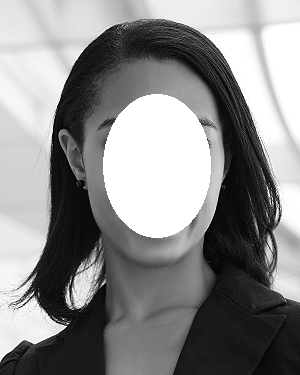
\includegraphics[width=1in,height=1.25in,clip,keepaspectratio]{author2.png}}]{Second
        B. Author} (M'76--SM'81--F'87) and all authors may include
    biographies. Biographies are often not included in conference-related
    papers. This author became a Member (M) of IEEE in 1976, a Senior
    Member (SM) in 1981, and a Fellow (F) in 1987. The first paragraph may
    contain a place and/or date of birth (list place, then date). Next,
    the author's educational background is listed. The degrees should be
    listed with type of degree in what field, which institution, city,
    state, and country, and year the degree was earned. The author's major
    field of study should be lower-cased.

    The second paragraph uses the pronoun of the person (he or she) and not the
    author's last name. It lists military and work experience, including summer
    and fellowship jobs. Job titles are capitalized. The current job must have
    a
    location; previous positions may be listed
    without one. Information concerning previous publications may be included.
    Try not to list more than three books or published articles. The format for
    listing publishers of a book within the biography is: title of book
    (publisher name, year) similar to a reference. Current and previous
    research
    interests end the paragraph.

    The third paragraph begins with the author's
    title and last name (e.g., Dr.\ Smith, Prof.\ Jones, Mr.\ Kajor, Ms.\
    Hunter).
    List any memberships in professional societies other than the IEEE.
    Finally,
    list any awards and work for IEEE committees and publications. If a
    photograph is provided, it should be of good quality, and
    professional-looking. Following are two examples of an author's biography.
\end{IEEEbiography}

\newpage

%If you do not have or do not want to include a photo, you can use IEEEbiographynophoto as shown below:

\begin{IEEEbiographynophoto}{Third C. Author, Jr.} (M'87) received the B.S.
    degree in mechanical
    engineering from National Chung Cheng University, Chiayi, Taiwan, in 2004
    and the M.S. degree in mechanical engineering from National Tsing Hua
    University, Hsinchu, Taiwan, in 2006. He is currently pursuing the Ph.D.
    degree in mechanical engineering at Texas A{\&}M University, College
    Station, TX, USA.

    From 2008 to 2009, he was a Research Assistant with the Institute of
    Physics, Academia Sinica, Tapei, Taiwan. His research interest includes the
    development of surface processing and biological/medical treatment
    techniques using nonthermal atmospheric pressure plasmas, fundamental study
    of plasma sources, and fabrication of micro- or nanostructured surfaces.

    Mr. Author's awards and honors include the Frew Fellowship (Australian
    Academy of Science), the I. I. Rabi Prize (APS), the European Frequency and
    Time Forum Award, the Carl Zeiss Research Award, the William F. Meggers
    Award and the Adolph Lomb Medal (OSA).
\end{IEEEbiographynophoto}

\EOD

\end{document}
